\subsection{Esquema del servidor}

    El esquema de servidor se basa en el patrón \emph{MVC} (Modelo, Vista, Controlador) que provee \emph{CodeIgniter} con su framework.

    El modo de funcionar este patrón es el siguiente:

        \begin{itemize}
            \item Un usuario lanza una petición contra la siguiente url

                http://www.example.com/clientes/get\_cliente/1

            \item A través del modulo mod\_rewrite se redirige la petición al fichero \emph{index.php} de CodeIgniter, el cual se encarga de analizar la petición siguiendo el siguiente flujo de trabajo:

            \begin{figure}[H]
                \centering
                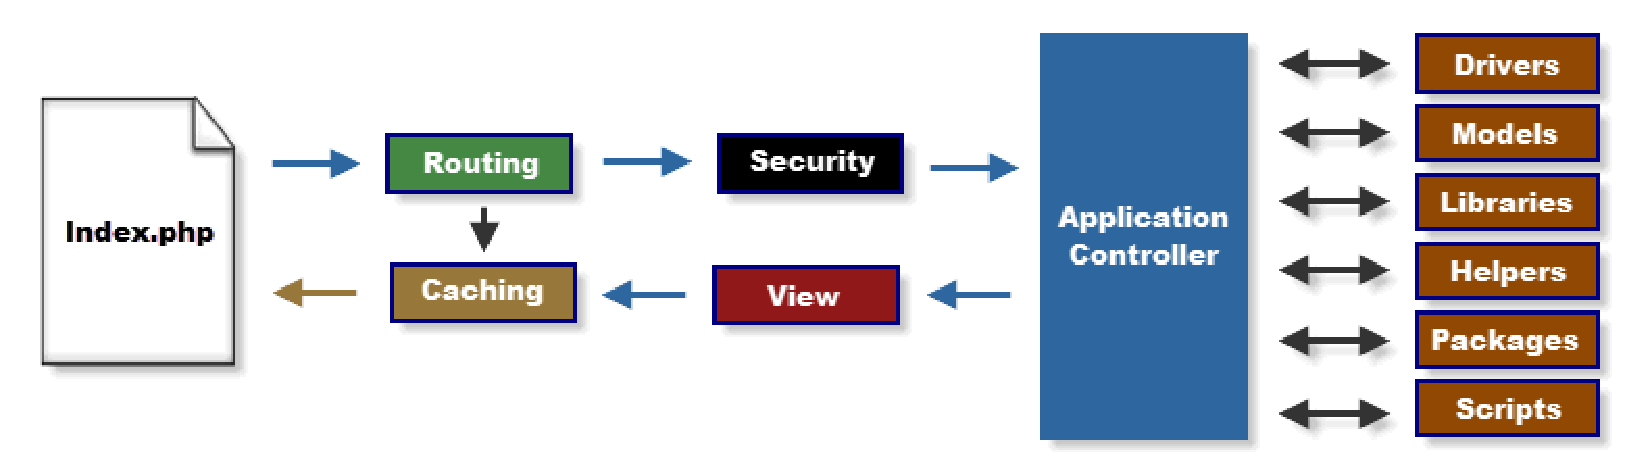
\includegraphics[keepaspectratio,width=0.9\textwidth]{flujo-trabajo-codeigniter.eps}
                \caption{Flujo de trabajo de CodeIgniter}\label{fig:flujo-trabajo-codeigniter}
            \end{figure}

            \item CodeIgniter descompone la URL en la siguiente estructura para conocer a que controlador tiene que pasar la petición, a que función llamar y qué parametros debe pasar.

                http://example.com/[controller-class]/[controller-method]/[arguments]

            Siendo para nuestro ejemplo los siguientes valores:

                \begin{itemize}
                    \item Controller class: clientes
                    \item Controller method: get\_cliente
                    \item Arguments: 1
                \end{itemize}
        \end{itemize}

    Los controladores son los encargados de procesar la petición, cargar tantas librerías, modelos... como necesiten para finalmente devolver un resultado.

    \subsubsection{Extendiendo el core de CodeIgniter}

    CodeIgniter al cargarse intenta buscar los sisguientes ficheros de sistema en la carpeta \emph{application/core}, esta funcionalidad permite sobreescribir algunas de las funcionalidades para ampliarlas.

    En el proyecto se han creado dos nuevos controladores para ampliar la funcionalidad del controlador por defecto de CodeIgniter:

    \begin{itemize}
        \item MY\_Controller

        Extiende de \emph{CI\_Controller} y se encarga de:

            \begin{itemize}
                \item Cargar la librería \emph{login\_auth} si no se están ejecutando los tests unitarios
                \item Ofrecer los siguientes métodos para renderizar la respuesta (\emph{\_renderJson}, \emph{\_renderXml}, \emph{\_renderToVar}, \emph{\_render})
            \end{itemize}

        \item MY\_Controller\_User

        Extiende de \emph{MY\_Controller} y únicamente se encarga de validar en el constructor que el usuario está logueado en el sistema, en caso de no estarlo, redirije a la Home pública.
    \end{itemize}

    \subsubsection{Esquema de controladores, modelos y librerías}